\newcommand*{\PaperRoot}{../../} %

%% bare_conf.tex
%% V1.3
%% 2007/01/11
%% by Michael Shell
%% See:
%% http://www.michaelshell.org/
%% for current contact information.
%%
%% This is a skeleton file demonstrating the use of IEEEtran.cls
%% (requires IEEEtran.cls version 1.7 or later) with an IEEE conference paper.
%%
%% Support sites:
%% http://www.michaelshell.org/tex/ieeetran/
%% http://www.ctan.org/tex-archive/macros/latex/contrib/IEEEtran/
%% and
%% http://www.ieee.org/

%%*************************************************************************
%% Legal Notice:
%% This code is offered as-is without any warranty either expressed or
%% implied; without even the implied warranty of MERCHANTABILITY or
%% FITNESS FOR A PARTICULAR PURPOSE! 
%% User assumes all risk.
%% In no event shall IEEE or any contributor to this code be liable for
%% any damages or losses, including, but not limited to, incidental,
%% consequential, or any other damages, resulting from the use or misuse
%% of any information contained here.
%%
%% All comments are the opinions of their respective authors and are not
%% necessarily endorsed by the IEEE.
%%
%% This work is distributed under the LaTeX Project Public License (LPPL)
%% ( http://www.latex-project.org/ ) version 1.3, and may be freely used,
%% distributed and modified. A copy of the LPPL, version 1.3, is included
%% in the base LaTeX documentation of all distributions of LaTeX released
%% 2003/12/01 or later.
%% Retain all contribution notices and credits.
%% ** Modified files should be clearly indicated as such, including  **
%% ** renaming them and changing author support contact information. **
%%
%% File list of work: IEEEtran.cls, IEEEtran_HOWTO.pdf, bare_adv.tex,
%%                    bare_conf.tex, bare_jrnl.tex, bare_jrnl_compsoc.tex
%%*************************************************************************

% *** Authors should verify (and, if needed, correct) their LaTeX system  ***
% *** with the testflow diagnostic prior to trusting their LaTeX platform ***
% *** with production work. IEEE's font choices can trigger bugs that do  ***
% *** not appear when using other class files.                            ***
% The testflow support page is at:
% http://www.michaelshell.org/tex/testflow/



% Note that the a4paper option is mainly intended so that authors in
% countries using A4 can easily print to A4 and see how their papers will
% look in print - the typesetting of the document will not typically be
% affected with changes in paper size (but the bottom and side margins will).
% Use the testflow package mentioned above to verify correct handling of
% both paper sizes by the user's LaTeX system.
%
% Also note that the "draftcls" or "draftclsnofoot", not "draft", option
% should be used if it is desired that the figures are to be displayed in
% draft mode.
%
\documentclass[10pt, conference, letterpaper]{IEEEtran}
% Add the compsoc option for Computer Society conferences.
%
% If IEEEtran.cls has not been installed into the LaTeX system files,
% manually specify the path to it like:
% \documentclass[conference]{../sty/IEEEtran}





% Some very useful LaTeX packages include:
% (uncomment the ones you want to load)


% *** MISC UTILITY PACKAGES ***
%
\usepackage{ifpdf}
% Heiko Oberdiek's ifpdf.sty is very useful if you need conditional
% compilation based on whether the output is pdf or dvi.
% usage:
% \ifpdf
%   % pdf code
% \else
%   % dvi code
% \fi
% The latest version of ifpdf.sty can be obtained from:
% http://www.ctan.org/tex-archive/macros/latex/contrib/oberdiek/
% Also, note that IEEEtran.cls V1.7 and later provides a builtin
% \ifCLASSINFOpdf conditional that works the same way.
% When switching from latex to pdflatex and vice-versa, the compiler may
% have to be run twice to clear warning/error messages.






% *** CITATION PACKAGES ***
%
%\usepackage{cite}
% cite.sty was written by Donald Arseneau
% V1.6 and later of IEEEtran pre-defines the format of the cite.sty package
% \cite{} output to follow that of IEEE. Loading the cite package will
% result in citation numbers being automatically sorted and properly
% "compressed/ranged". e.g., [1], [9], [2], [7], [5], [6] without using
% cite.sty will become [1], [2], [5]--[7], [9] using cite.sty. cite.sty's
% \cite will automatically add leading space, if needed. Use cite.sty's
% noadjust option (cite.sty V3.8 and later) if you want to turn this off.
% cite.sty is already installed on most LaTeX systems. Be sure and use
% version 4.0 (2003-05-27) and later if using hyperref.sty. cite.sty does
% not currently provide for hyperlinked citations.
% The latest version can be obtained at:
% http://www.ctan.org/tex-archive/macros/latex/contrib/cite/
% The documentation is contained in the cite.sty file itself.






% *** GRAPHICS RELATED PACKAGES ***
%
\ifCLASSINFOpdf
  \usepackage[pdftex]{graphicx}
  % declare the path(s) where your graphic files are
  \graphicspath{{../pdf/}{../jpeg/}}
  % and their extensions so you won't have to specify these with
  % every instance of \includegraphics
  \DeclareGraphicsExtensions{.pdf,.jpeg,.png}
\else
  % or other class option (dvipsone, dvipdf, if not using dvips). graphicx
  % will default to the driver specified in the system graphics.cfg if no
  % driver is specified.
  \usepackage[dvips]{graphicx}
  % declare the path(s) where your graphic files are
  \graphicspath{{../eps/}}
  % and their extensions so you won't have to specify these with
  % every instance of \includegraphics
  \DeclareGraphicsExtensions{.eps}
\fi
% graphicx was written by David Carlisle and Sebastian Rahtz. It is
% required if you want graphics, photos, etc. graphicx.sty is already
% installed on most LaTeX systems. The latest version and documentation can
% be obtained at: 
% http://www.ctan.org/tex-archive/macros/latex/required/graphics/
% Another good source of documentation is "Using Imported Graphics in
% LaTeX2e" by Keith Reckdahl which can be found as epslatex.ps or
% epslatex.pdf at: http://www.ctan.org/tex-archive/info/
%
% latex, and pdflatex in dvi mode, support graphics in encapsulated
% postscript (.eps) format. pdflatex in pdf mode supports graphics
% in .pdf, .jpeg, .png and .mps (metapost) formats. Users should ensure
% that all non-photo figures use a vector format (.eps, .pdf, .mps) and
% not a bitmapped formats (.jpeg, .png). IEEE frowns on bitmapped formats
% which can result in "jaggedy"/blurry rendering of lines and letters as
% well as large increases in file sizes.
%
% You can find documentation about the pdfTeX application at:
% http://www.tug.org/applications/pdftex





% *** MATH PACKAGES ***
%
\usepackage[cmex10]{amsmath}
% A popular package from the American Mathematical Society that provides
% many useful and powerful commands for dealing with mathematics. If using
% it, be sure to load this package with the cmex10 option to ensure that
% only type 1 fonts will utilized at all point sizes. Without this option,
% it is possible that some math symbols, particularly those within
% footnotes, will be rendered in bitmap form which will result in a
% document that can not be IEEE Xplore compliant!
%
% Also, note that the amsmath package sets \interdisplaylinepenalty to 10000
% thus preventing page breaks from occurring within multiline equations. Use:
\interdisplaylinepenalty=2500
% after loading amsmath to restore such page breaks as IEEEtran.cls normally
% does. amsmath.sty is already installed on most LaTeX systems. The latest
% version and documentation can be obtained at:
% http://www.ctan.org/tex-archive/macros/latex/required/amslatex/math/





% *** SPECIALIZED LIST PACKAGES ***
%
%\usepackage{algorithmic}
% algorithmic.sty was written by Peter Williams and Rogerio Brito.
% This package provides an algorithmic environment fo describing algorithms.
% You can use the algorithmic environment in-text or within a figure
% environment to provide for a floating algorithm. Do NOT use the algorithm
% floating environment provided by algorithm.sty (by the same authors) or
% algorithm2e.sty (by Christophe Fiorio) as IEEE does not use dedicated
% algorithm float types and packages that provide these will not provide
% correct IEEE style captions. The latest version and documentation of
% algorithmic.sty can be obtained at:
% http://www.ctan.org/tex-archive/macros/latex/contrib/algorithms/
% There is also a support site at:
% http://algorithms.berlios.de/index.html
% Also of interest may be the (relatively newer and more customizable)
% algorithmicx.sty package by Szasz Janos:
% http://www.ctan.org/tex-archive/macros/latex/contrib/algorithmicx/




% *** ALIGNMENT PACKAGES ***
%
%\usepackage{array}
% Frank Mittelbach's and David Carlisle's array.sty patches and improves
% the standard LaTeX2e array and tabular environments to provide better
% appearance and additional user controls. As the default LaTeX2e table
% generation code is lacking to the point of almost being broken with
% respect to the quality of the end results, all users are strongly
% advised to use an enhanced (at the very least that provided by array.sty)
% set of table tools. array.sty is already installed on most systems. The
% latest version and documentation can be obtained at:
% http://www.ctan.org/tex-archive/macros/latex/required/tools/


\usepackage{mdwmath}
\usepackage{mdwtab}
% Also highly recommended is Mark Wooding's extremely powerful MDW tools,
% especially mdwmath.sty and mdwtab.sty which are used to format equations
% and tables, respectively. The MDWtools set is already installed on most
% LaTeX systems. The lastest version and documentation is available at:
% http://www.ctan.org/tex-archive/macros/latex/contrib/mdwtools/


% IEEEtran contains the IEEEeqnarray family of commands that can be used to
% generate multiline equations as well as matrices, tables, etc., of high
% quality.


%\usepackage{eqparbox}
% Also of notable interest is Scott Pakin's eqparbox package for creating
% (automatically sized) equal width boxes - aka "natural width parboxes".
% Available at:
% http://www.ctan.org/tex-archive/macros/latex/contrib/eqparbox/





% *** SUBFIGURE PACKAGES ***
%\usepackage[tight,footnotesize]{subfigure}
% subfigure.sty was written by Steven Douglas Cochran. This package makes it
% easy to put subfigures in your figures. e.g., "Figure 1a and 1b". For IEEE
% work, it is a good idea to load it with the tight package option to reduce
% the amount of white space around the subfigures. subfigure.sty is already
% installed on most LaTeX systems. The latest version and documentation can
% be obtained at:
% http://www.ctan.org/tex-archive/obsolete/macros/latex/contrib/subfigure/
% subfigure.sty has been superceeded by subfig.sty.



%\usepackage[caption=false]{caption}
%\usepackage[font=footnotesize]{subfig}
% subfig.sty, also written by Steven Douglas Cochran, is the modern
% replacement for subfigure.sty. However, subfig.sty requires and
% automatically loads Axel Sommerfeldt's caption.sty which will override
% IEEEtran.cls handling of captions and this will result in nonIEEE style
% figure/table captions. To prevent this problem, be sure and preload
% caption.sty with its "caption=false" package option. This is will preserve
% IEEEtran.cls handing of captions. Version 1.3 (2005/06/28) and later 
% (recommended due to many improvements over 1.2) of subfig.sty supports
% the caption=false option directly:
\usepackage[caption=false,font=footnotesize]{subfig}
%
% The latest version and documentation can be obtained at:
% http://www.ctan.org/tex-archive/macros/latex/contrib/subfig/
% The latest version and documentation of caption.sty can be obtained at:
% http://www.ctan.org/tex-archive/macros/latex/contrib/caption/




% *** FLOAT PACKAGES ***
%
%\usepackage{fixltx2e}
% fixltx2e, the successor to the earlier fix2col.sty, was written by
% Frank Mittelbach and David Carlisle. This package corrects a few problems
% in the LaTeX2e kernel, the most notable of which is that in current
% LaTeX2e releases, the ordering of single and double column floats is not
% guaranteed to be preserved. Thus, an unpatched LaTeX2e can allow a
% single column figure to be placed prior to an earlier double column
% figure. The latest version and documentation can be found at:
% http://www.ctan.org/tex-archive/macros/latex/base/



%\usepackage{stfloats}
% stfloats.sty was written by Sigitas Tolusis. This package gives LaTeX2e
% the ability to do double column floats at the bottom of the page as well
% as the top. (e.g., "\begin{figure*}[!b]" is not normally possible in
% LaTeX2e). It also provides a command:
%\fnbelowfloat
% to enable the placement of footnotes below bottom floats (the standard
% LaTeX2e kernel puts them above bottom floats). This is an invasive package
% which rewrites many portions of the LaTeX2e float routines. It may not work
% with other packages that modify the LaTeX2e float routines. The latest
% version and documentation can be obtained at:
% http://www.ctan.org/tex-archive/macros/latex/contrib/sttools/
% Documentation is contained in the stfloats.sty comments as well as in the
% presfull.pdf file. Do not use the stfloats baselinefloat ability as IEEE
% does not allow \baselineskip to stretch. Authors submitting work to the
% IEEE should note that IEEE rarely uses double column equations and
% that authors should try to avoid such use. Do not be tempted to use the
% cuted.sty or midfloat.sty packages (also by Sigitas Tolusis) as IEEE does
% not format its papers in such ways.





% *** PDF, URL AND HYPERLINK PACKAGES ***
%
\usepackage{url}
% url.sty was written by Donald Arseneau. It provides better support for
% handling and breaking URLs. url.sty is already installed on most LaTeX
% systems. The latest version can be obtained at:
% http://www.ctan.org/tex-archive/macros/latex/contrib/misc/
% Read the url.sty source comments for usage information. Basically,
% \url{my_url_here}.





% *** Do not adjust lengths that control margins, column widths, etc. ***
% *** Do not use packages that alter fonts (such as pslatex).         ***
% There should be no need to do such things with IEEEtran.cls V1.6 and later.
% (Unless specifically asked to do so by the journal or conference you plan
% to submit to, of course. )


% correct bad hyphenation here
\hyphenation{op-tical net-works semi-conduc-tor}

\graphicspath{{../pdf/}{../jpeg/}{img/}{../../../Figures/}}
\usepackage{todonotes}
\usepackage{booktabs}

\begin{document}
%
% paper title
% can use linebreaks \\ within to get better formatting as desired
\title{Multi-Domain Trust Frameworks for Harsh Environments}


% author names and affiliations
% use a multiple column layout for up to three different
% affiliations
\author{\IEEEauthorblockN{Andrew Bolster}
\IEEEauthorblockA{Department of Electrical Engineering and Electronics\\
University of Liverpool\\
Liverpool, UK\\
Email: andrew.bolster@liverpool.ac.uk}
\and
\IEEEauthorblockN{Alan Marshall}
\IEEEauthorblockA{Department of Electrical Engineering and Electronics\\
University of Liverpool\\
Liverpool, UK\\
Email: alan.marshall@liverpool.ac.uk}
}
% conference papers do not typically use \thanks and this command
% is locked out in conference mode. If really needed, such as for
% the acknowledgment of grants, issue a \IEEEoverridecommandlockouts
% after \documentclass

% for over three affiliations, or if they all won't fit within the width
% of the page, use this alternative format:
% 
%\author{\IEEEauthorblockN{Michael Shell\IEEEauthorrefmark{1},
%Homer Simpson\IEEEauthorrefmark{2},
%James Kirk\IEEEauthorrefmark{3}, 
%Montgomery Scott\IEEEauthorrefmark{3} and
%Eldon Tyrell\IEEEauthorrefmark{4}}
%\IEEEauthorblockA{\IEEEauthorrefmark{1}School of Electrical and Computer Engineering\\
%Georgia Institute of Technology,
%Atlanta, Georgia 30332--0250\\ Email: see http://www.michaelshell.org/contact.html}
%\IEEEauthorblockA{\IEEEauthorrefmark{2}Twentieth Century Fox, Springfield, USA\\
%Email: homer@thesimpsons.com}
%\IEEEauthorblockA{\IEEEauthorrefmark{3}Starfleet Academy, San Francisco, California 96678-2391\\
%Telephone: (800) 555--1212, Fax: (888) 555--1212}
%\IEEEauthorblockA{\IEEEauthorrefmark{4}Tyrell Inc., 123 Replicant Street, Los Angeles, California 90210--4321}}




% use for special paper notices
%\IEEEspecialpapernotice{(Invited Paper)}




% make the title area
\maketitle


\begin{abstract}
%\boldmath
With the increasing application of autonomy in cyber-physical systems, Trust Management Frameworks (TMFs) are being used to improve the efficiency, security, and reliability of decentralized and distributed autonomous systems. 
In such systems, subtle misbehaviors can significantly impact the operation and performance of the system as a whole. Techniques have been developed for high-speed, uncontended environments such as terrestrial 802.11 MANETs. 
However, these do not perform well in sparse / harsh environments such as those found in Underwater Acoustic Networks (UANs), where network nodes experience significant and variable delays, comparatively low data rates, large contention periods, and considerable multi-path artifacts. 
In such sparse networks, trust establishment based on statistical observations of success/failure events become unstable and ineffective in detecting or identifying misbehaviors. 
Additionally, these methodologies focus solely on the communications actions of entities and do not incorporate the physical domain. 
In this paper we demonstrate the use and operation of a multi-domain trust management framework (MD-TMF) for collaborative mobile autonomous networks (CMANs), using UANs as an exemplar application. 
In this paper we demonstrate a methodology that applies Grey Sequence operations and Grey Generators (conceptually analogous to Sequential Bayesian Filtering``) to provide continuous trust assessment in a sparse, asynchronous metric space across multiple domains of trust.
We also present a machine learning methodology for assessing the relative and collective performance of varying metric sets and subsets in detection and differentiation of a range of communications and physical misbehaviors.

\end{abstract}
% IEEEtran.cls defaults to using nonbold math in the Abstract.
% This preserves the distinction between vectors and scalars. However,
% if the conference you are submitting to favors bold math in the abstract,
% then you can use LaTeX's standard command \boldmath at the very start
% of the abstract to achieve this. Many IEEE journals/conferences frown on
% math in the abstract anyway.

% no keywords




% For peer review papers, you can put extra information on the cover
% page as needed:
% \ifCLASSOPTIONpeerreview
% \begin{center} \bfseries EDICS Category: 3-BBND \end{center}
% \fi
%
% For peerreview papers, this IEEEtran command inserts a page break and
% creates the second title. It will be ignored for other modes.
\IEEEpeerreviewmaketitle



\section{Introduction}
% no \IEEEPARstart
With the increasing application of autonomy in cyber-physical systems, Trust Management Frameworks (TMFs) are increasingly being applied to assist the efficiency, security, and reliability of decentralised and distributed autonomous systems, from highway-bound autonomous vehicles to aerial battlefield drones. 
Classical applications of trust management in Mobile Ad-Hoc Networks (MANETs) have focused solely on observations from the communications domain to make trust assessments. 
However, these methods are not as effective in applications exhibiting sparse, delayed, or otherwise challenged communications environments\cite{Pavan2015}. MD-TMF expands this paradigm to include relevant physical factors and movements to increase the threat area covered the trust framework. An example area of application is the underwater marine environment, where extreme challenges to communications present themselves (propagation delays, frequency dependent attenuation, fast and slow fading, refractive multi-path distortion, etc.).
In addition to the communications challenges, other considerations such as command and control isolation, as well as power and locomotive limitations, drive towards the use of teams of smaller and cheaper autonomous underwater vehicles (AUVs). These increasingly decentralised applications present unique threats against trust management. In underwater environments, communications is both sparse and noisy.
Therefore the observations about the communications processes that are used to generate the trust metrics, occur much less frequently, with much greater error (noise) and delay than is experienced in terrestrial RF MANETS.
Trust Management Frameworks (TMFs) provide information to assist the estimation of future states and actions of nodes within networks. This information is used to optimize the performance of a network against malicious, selfish, or defective misbehaviour by one or more nodes. Previous research has established the advantages of implementing TMFs in 802.11 based MANETs, particularly in terms of preventing selfish operation in collaborative systems \cite{Li2007}, and maintaining throughput in the presence of malicious actors \cite{Buchegger2002}. Most current TMFs use a single type of observed action to derive trust values, typically successfully delivered or forwarded packets. These observations then inform future decisions of individual nodes, for example, route selection \cite{Li2008}.
Recent work has demonstrated the use of a number of metrics to form a ``vector'' of trust. The Multi-parameter Trust Framework for MANETs (MTFM) \cite{Guo11}, uses a range of communications metrics beyond packet delivery/loss rate (PLR) to assess trust. This vectorized trust also allows a system to detect and identify the tactics being used to undermine or subvert trust. The authors have previously applied this method to the marine space, comparing against a selection of existing communications TMFs \cite{Bolster2015b} showing that MTFM is more effective at detecting misbehaviours in sparse environments. This paper continues and extends that work to encompass physical as well as communications observations in the establishment of trust and the detection and classification of misbehaviours across both physical and communications domains. 
This paper is laid out as follows; in section 2 we discuss Trust and TMFs, defining out terminology and reviewing the justifications for the use and development of TMFs in harsh environments such as UANs.
In section 3 we review selected features of the underwater communications channel, highlighting particular challenges against terrestrial equivalents. 
In section 4 we review the findings of \cite{Bolster2015b} and establish experimental parameters and simulated behaviours under assessment. 
In section 5 we present our analysis pipeline for assessing misbehaviour using MTFM, and intermediate results of the independent detection of physical and communications misbehaviours using single-domain observations. 
In section 6 we demonstrate results from multi-domain MTFM and discuss the significance of these findings in terms of detection and classification of cross-domain misbehaviour sets.

\section{Trust and Trust Management Frameworks}

\subsubsection{Trust in Networked Systems}

\begin{figure}[h!]
	\centering
	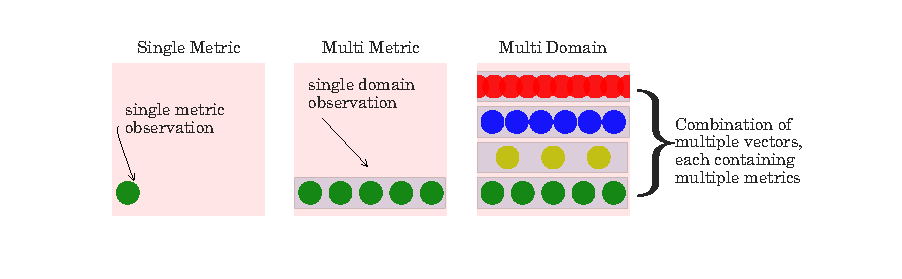
\includegraphics[width=0.9\linewidth]{threat_surface_sum}
	
	\caption{With the addition of further metrics, the threat surface available to an attacker is greatly reduced}
\end{figure}
\todo[inline]{Insert Generic Discussion of Trust Here: ¼ pg}

\subsection{Trust Management in Conventional MANETs}
The distributed and dynamic nature of MANETs mean that it is difficult to maintain a trusted third party (TTP) or evidence based trust system such as Certificate Authorities (CA) or Public Key Infrastructure (PKI). 
Distributed trust management frameworks aim to detect, identify, and mitigate the impacts of malicious actors by distributing per-node assessments and opinions to collectively police behaviour. 
Various models and algorithms for describing trust and developing trust management in distributed systems, P2P communities or wireless networks have been considered.
\textit{Hermes Trust Establishment Framework} uses a Bayesian Beta function to model per-link Packet Loss Rate (PLR) over time, combining ``Trust'' and ``Confidence of Assessment'' into a single value \cite{Zouridaki2005}.
\textit{Objective Trust Management Framework} (OTMF) builds upon Hermes and distributes node observations across the network \cite{Li2008}, however does not appropriately combat multi-node-collusion in the network \cite{Cho2011}. 
\textit{Trust-based Secure Routing} demonstrated an extension to Dynamic Source Routing (DSR), incorporating a Hidden Markov Model of sub-networks, reducing the efficacy of Byzantine attacks such as black-hole routing  \cite{Moe2008a}. 
\textit{CONFIDANT} presented an approach using a probabilistic estimation of PLR, similar to OTMF, also introducing a topology aware weighting scheme and also weighting trust assessments based on historical experience of the reporter \cite{Buchegger2002}. Fuzzy Trust-Based Filtering uses Fuzzy Inference to adapt to malicious recommenders using conditional similarity to classify performance with overlapping fuzzy set membership, filtering assessments across a network \cite{Luo2008}. 
These TMFs can be generalised as single-value estimation based on a binary input state (success or failure of packet delivery) and generating a probabilistic estimation of the future states of that input. These single metric TMFs provide malicious actors with a significant advantage if their activity does not impact that metric.In the case where the attacker can subvert the TMF, the metric under assessment by that TMF does not cover the threat mounted by the attacker. This causes a significant negative effect on the efficiency of the network, as the TMF is assumed to have reduced the possible set of attacks when it has actually made it more advantageous to attack a different part of the networks operation.
An example of such a situation would be in a TMF focused on PLR where an attacker selectively delays packets going through it, reducing overall throughput but not dropping any packets. Such behaviour would not be detected by the TMF.

As an example; The Hermes trust establishment framework \cite{Zouridaki2005} uses Bayesian reasoning to generate a posterior distribution function of ``belief'', or trust, given a sequence of observations of that behaviour, $p(B|O)$\eqref{eq:otmf_pbo}.

\begin{equation}
p(B|O)  = \frac{p(O|B) \times p(B)}{\rho}
\label{eq:otmf_pbo}
\end{equation}

Where $p(B)$ is the prior probability density function for the expected normal behaviour, and $\rho$ is a normalising factor.
Due to it's flexibility and simplicity, Hermes assumes that $p(B)$ is a Beta function, and therefore the evaluation of this trust assessment is based around the expectation value of the distribution \eqref{eq:otmf_t}  where $\alpha$ and $\beta$ represent the number of successful and unsuccessful interactions respectively for a particular node $i$.

A secondary measurement of the confidence factor of the trust assessment $t$ is generated as \eqref{eq:otmf_c} and these measurements are combined to form a ``trustworthiness'' value $T$ \eqref{eq:otmf_trust}.

\begin{align}
t_i &\to E\lbrack\text{beta}(p|\alpha,\beta)\rbrack = \frac{\alpha_i}{\alpha_i+\beta_i} \label{eq:otmf_t}\\[5pt]
c_i &= 1 - \sqrt{\frac{12\alpha_i\beta_i}{(\alpha_i+\beta_i)^2(\alpha_i+\beta_i+1)}} \label{eq:otmf_c}\\[5pt]
T_i &= 1 - \frac{\sqrt{\frac{(t_i-1)^2}{x^2} + \frac{(c_i-1)^2}{y^2}}}{\sqrt{\frac{1}{x^2}+\frac{1}{y^2}}} \label{eq:otmf_trust}
\end{align}

In \eqref{eq:otmf_trust}, $x$ and $y$ are constants, used weight the two-dimensional polar mapping of trust and confidence assessments ($t_i,c_i$), and from \cite{Zouridaki2005}, are taken as $x=\sqrt{2},y=\sqrt{9}$.

Upon this per-node assessment methodology, OTMF overlays an observation distribution protocol so as to make the measurements $\alpha_i$ and $\beta_i$ representative of the direct and 1-hop networks observations of the target node $i$, as well as expiring old observations from assessment and eliminating observations from ``untrustworthy'' nodes.


\textit{Multi-Parameter Trust Framework for MANETS} (MTFM) extends this single-parameter approach, applying Grey Relational Analysis \cite{Zuo1995} to provide cohort based normalization of a range of disparate metrics at runtime, providing a “grade” of trust compared to other observed nodes, while maintaining the ability to reduce trust valued down to a stable assessment range for decision support without requiring a-priori environmental or metric characterisation. This presents a stark difference between the previously discussed probabilistic approaches. Grey assessments are relative in both fairly and unfairly operating networks. All nodes will receive mid-range trust assessments if there are no malicious actors as there is nothing ``bad'' to compare against, and variations in assessment will be primarily driven by topological and environmental factors.
Guo et al. \cite{Guo11} demonstrated the ability of grey relational analysis (GRA) \cite{Zuo1995} to normalise and combine disparate traits of a communications link such as instantaneous throughput, received signal strength, etc. into a grey relational coefficient (GRC), or a ``trust vector'' in this instance.

The grey relational vector is given as
%
\begin{align}
\label{eq:grc}
\theta_{k,j}^t = \frac{\min_k|a_{k,j}^t - g_j^t| + \rho \max_k|a_{k,j}^t-g_j^t|}{|a_{k,j}^t-g_j^t| + \rho \max_k|a_{k,j}^t-g_j^t|} \\
\phi_{k,j}^t = \frac{\min_k|a_{k,j}^t - b_j^t| + \rho \max_k|a_{k,j}^t-b_j^t|}{|a_{k,j}^t-b_j^t| + \rho \max_k|a_{k,j}^t-b_j^t|} \notag 
\end{align}
%
where $a_{k,j}^t$ is the value of an observed metric $x_j$ for a given node $k$ at time $t$, $\rho$ is a distinguishing coefficient set to $0.5$, $g$ and $b$ are respectively the ``good'' and ``bad'' reference metric sequences from $\{a_{k,j}^t k=1,2\dots K\}$, i.e. $g_j=\max_k({a_{k,j}^t})$,  $b_j=\min_k({a_{k,j}^t})$ (where each metric is selected to be monotonically positive for trust assessment, e.g. higher throughput is presumed to be always better). 

Weighting can be applied before generating a scalar value \eqref{eq:metric_weighting} allowing the detection and classification of misbehaviours.

%
\begin{equation}
\label{eq:metric_weighting}
[\theta_k^t, \phi_k^t] = \left[\sum_{j=0}^M h_j \theta_{k,j}^t,\sum_{j=0}^M h_j \phi_{k,j}^t \right]
\end{equation}
%
Where $H=[h_0\dots h_M]$ is a metric weighting vector such that $\sum h_j = 1$, and in unweighted case, $H=[\frac{1}{M},\frac{1}{M}\dots\frac{1}{M}]$.
$\theta$ and $\phi$ are then scaled to $[0,1]$ using the mapping $y = 1.5 x - 0.5$.
To minimise the uncertainties of belonging to either best ($g$) or worst ($b$) sequences in \eqref{eq:grc} the $[\theta,\phi]$ values are reduced into a scalar trust value by $T_k^t = ({1+{(\phi_k^t)^2}/{(\theta_k^t)^2}})^{-1}$ \cite{Hong2010}.
MTFM combines this GRA with a topology-aware weighting scheme \eqref{eq:networkeffects} and a fuzzy whitenization model \eqref{eq:whitenization}. 

There are three classes of topological trust relationship used; Direct, Recommendation, and Indirect.
Where an observing node $n_i$ assesses the trust of another target node, $n_j$; the Direct relationship is $n_i$'s own observations $n_j$'s behaviour.
In the Recommendation case, a node $n_k$ which shares Direct relationships with both $n_i$ and $n_j$, gives its assessment of $n_j$ to $n_i$.
In the Indirect case, similar to the Recommendation case, the recommender $n_k$ does not have a direct link with the observer $n_i$ but $n_k$ has a Direct link with the target node, $n_j$.
These relationships give node sets, $N_R$ and $N_I$ containing the nodes that have recommendation or indirect, relationships to the observing node respectively.
%
\begin{align}
\label{eq:networkeffects}
T_{i,j}^{MTFM}=&\frac{1}{2} \cdot \max_s\{f_s(T_{i,j})\} T_{i,j}\\ \notag
+&\frac{1}{2} \frac{2|N_R| }{2|N_R| + |N_I|}\sum_{n \in N_R} \max_s\{f_s(T_{i,n})\} T_{i,n}\\ \notag
+&\frac{1}{2} \frac{|N_I| }{2|N_R| + |N_I|}\sum_{n \in N_I} \max_s\{f_s(T_{i,n})\} T_{i,n} 
\end{align}

Where $T_{i,n}$ is the subjective trust assessment of $n_i$ by $n_n$, and $f_s = [ f_1,f_2, f_3]$ given as:

\begin{align}
\label{eq:whitenization}
f_1(x)&= -x+1\notag\\
f_2(x)&= 
\begin{cases}
2x & \text{if }x\leq 0.5\\
-2x+2 & \text{if }x>0.5
\end{cases}\\
f_3(x)&= x\notag
\end{align}
%
In the case of the terrestrial communications network used in \cite{Guo11}, the observed metric set $X = {x_1,\dots,x_M}$ representing the measurements taken by each node of its neighbours at least interval, is defined as $X=[$packet loss rate, signal strength, data rate, delay, throughput$]$.

Guo et al. demonstrated that when compared against OTMF and Hermes trust assessment, MTFM provided increased variation in trust assessment over time, providing more information about the nodes' behaviours than packet delivery probability alone can.
By weighting the metrics used in MTFM it was shown that the trust assessments could be used to identify the style of misbehaviour being performed within the network, and by whom.
It has been demonstrated that MTFM is a strong candidate for trust assessment in the harsh marine communications environment \cite{Bolster2015b}.

\subsection{Multi-Metric Single Domain Trust in Harsh Environments}

It has been demonstrated that classical, single metric, MANET Trust Management Frameworks are not directly suitable to the sparse, noisy, and dynamic underwater medium, however MTFM shows promise in it's multi-metric normalisation approach when compared to the performance of OTMF and Hermes in the same scenarios \cite{Bolster2015b}.
In a simulated underwater environment, MTFM was able to discriminate between communications behaviours using communications metrics by exploring the metric space by weight variation, allowing the detection and classification of the malicious behaviours.
With significant delays (from seconds to many minutes), in a fading, refractive medium with varying propagation characteristics, the environment is not as predictable or performant as classical MANET TMF deployment environments. 
Without significant adaptation, single metric probabilistic estimation based TMFs are ineffective in such an environment.
Existing frameworks are overly optimistic about the nature and stability of the communications channel, and can overlook characteristics that are useful for assessing the behaviour of nodes in the network. 
This indicates that there is a good case, particularly within constrained MANETs as this for multi-domain trust assessment, where metrics about the communications network and topology are be brought together with information about the physical behaviours and operations of nodes to assess trust.




\section{Marine Acoustic Communications}

The key challenges of underwater acoustic communications are centred around the impact of slow and differential propagation of energy (RF, Optical, Acoustic) through water, and its interfaces with the seabed / air.
The resultant challenges include; long propagation delays, significant inter-symbol interference and Doppler spreading, fast and slow fading due to environmental effects (aquatic flora/fauna, surface weather), carrier-frequency dependent signal attenuation, multi-path caused by reflective medium interfaces, variations in propagation speed due to depth dependant effects (salinity, temperature, and pressure), and subsequent refractive spreading and lensing due to that same propagation variation \cite{Partan2006}.


The attenuation that occurs in an underwater acoustic channel over a distance $d$ for a signal about frequency $f$ in linear power is given as $A_{\text{aco}}(d,f) = A_0d^ka(f)^d$ and in $dB$ form as;
%
\begin{equation}
\label{eq:acoattenuationdb}
10 \log A_{\text{aco}}(d,f)/A_0 = k \cdot 10 \log d + d \cdot 10 \log a(f)
\end{equation}
%
where $A_0$ is a normalising constant, $k$ is a spreading factor (commonly taken as 1.5  \cite{Stojanovic2007}), and $a(f)$ is the absorption coefficient, approximated using Thorp's formula \cite{Stefanov2011}
%
\begin{equation}
\label{eq:thorp}
10 \log a(f) = \frac{0.11 \cdot f^2}{1+f^2} + \frac{44\cdot f^2}{4100+f^2}+ 2.75\times10^{-4} f^2 + 0.003
\end{equation}
%

Refractive lensing and the multi-path nature of the medium result in line of sight propagation being extremely unreliable for estimating distances to targets.
The first arriving acoustic signal has as the very least curved in the medium, and commonly has reflected off the surface/seabed before arriving at a receiver, creating secondary paths that are sometimes many times longer than the first arrival path, generating symbol spreading over orders of seconds depending on the ranges and depths involved.
Forward Error Correction coding is used on such channels to minimise packet losses.

Comparing $A_{aco}(d,f)$ with the RF Free-Space Path Loss model $(A_{\text{RF}}(d,f) \approx \left( \frac{4\pi d f}{c} \right)^2)$, the impact of range on signal power is exponential underwater, rather than quadratic in terrestrial RF ($A_{\text{aco}} \propto f^{2d}$ vs $A_{\text{RF}} \propto (df)^2$). 
While both frequency dependant factors are quadratic, approximating the factors in \eqref{eq:thorp}, $f\propto A_{\text{aco}}$ is at least 4 orders of magnitude higher than $f\propto A_{\text{RF}}$

\section{Analysis Design and Per-Domain Results}


\subsection{Simulation and Scenario Generation}
To investigate the operation of a fully mobile network of six nodes, each kinematically modelled on the REMUS 100 \cite{Milgram2001} in the marine environment, simulations were conducted using a Python based framework, SimPy \cite{Mueller2003SimPy}, with a network stack built upon AUVNetSim \cite{Miquel2008}, using transmission parameters (Table \ref{tab:sysconstraints}) taken from and validated against \cite{Stojanovic2007} and \cite{Stefanov2011}.

Four misbehaviours were developed to assess both communications and physical misbehaviours \todo{check that we actually talk about misbehaviours before this} such that one node within the fleet was 'misbehaving' ($n_m$). In cases where $n_m$ is specifically targeting another node in the fleet, that node is denoted as $n_t$.

\begin{enumerate}
	\item Malicious Power Control (MPC), where $n_m$ increases its transmit and forwarding power by 20\% for all nodes \emph{except} communications from $n_t$ in order to make $n_t$ appear to be selfishly conserving energy to the rest of the team, while $n_t$ itself appears to be performing very well.
	\item Selfish Target Selection (STS), where $n_m$ preferentially communicates, forwards and advertises to nodes that are physically close to it in effort to reduce its own power consumption.
	\item Shadowing, where $n_m$ is not aware of the pre-planned mission paths and is instead simply following it's neighbours. \todo{This is really bad; this may not apply in this mobility constraint}
	\item Slow Coach, where $n_m$ is experiencing a simulated power-train failure that reduces it's acceleration and top speed, analogous to a fouled propeller. 
\end{enumerate}

The default scenario is also simulated where nodes participate fairly in the network and follow a collaborative survey mobility pattern.

From these simulations, we attain the per-node recorded positions, ($P_i = [x,y,z] \forall t$) as well as each nodes estimations of it's neighbours positions $P_{i,j} = [x,y,z] \forall t$) (which assumes that all nodes are fairly operating their positions compactly at each transmission), and each nodes trust metric observations of it's neighbours; $A_{i,j}^t = [ x_{i,j} \forall x \in X ] $ where $X$ are the selected trust metrics.

%
\begin{table}[h]
	\caption{Comparison of system model constraints as applied between Terrestrial and Marine communications} \label{tab:sysconstraints}
	\begin{center}
		\setlength{\tabcolsep}{8pt}
		\begin{tabular}{lccc}
			\toprule
			Parameter & Unit & Terrestrial & Marine \\
			\midrule
			Simulated Duration & $s$ & 300 & 18000\\
			Initial Node Separation & $100m$ & $300m$\\
			Trust Sampling Period & $s$ & 1 & 600 \\
			Simulated Area & $km^2$ & 0.7 & 0.7-4 \\
			Transmission Range & $km$ & 0.25 & 1.5 \\
			Physical Layer & & RF(802.11) & Acoustic\\
			Propagation Speed& $m/s$ & $3\times10^8$ & 1490\\
			Center Frequency& $Hz$ & $2.6\times10^9$ & $2 \times 10^4$ \\
			Bandwidth& $Hz$ & $22\times10^6$ & $1\times10^4$\\
			MAC Type & & CSMA/DCF & CSMA/CA\\
			Routing Protocol & & DSDV & FBR \\
			Max Speed & $ms^{-1}$ & 5 & 1.5 \\
			Max Data Rate & $bps$ & $5\times10^6$ & $\approx 240$ \\
			Packet Size & bits & 4096 &  9600 \\
			Single Transmission Duration & $s$ & 10 & 32 \\
			Single Transmission Size & bits & $10^7$ & $9600$ \\
			\bottomrule
		\end{tabular}
		\setlength{\tabcolsep}{6pt}
	\end{center}
\end{table}
%

\subsection{Communications Trust Metrics}

We use the same metrics from \cite{Guo2012} that are applicable to the marine environment, i.e. as the simulated modem stack does not operate on the same tiered data-rate approach as used in the 802.11 stack, that metric was not included. Remaining metrics are; Delay, Received and Transmitted power, Received and Transmitted Throughput, and Packet Loss Rate (PLR).

\subsection{Behavioural Trust Metrics}

Three physical metrics are selected to encompass the relative distributions and activities of nodes within the network; Inter-Node Distance Deviation (INDD), Inter-Node Heading Deviation (INHD), and Node Speed. These metrics encapsulate the relative distributions of position and velocity within the fleet, optimising for the detection of outlying or deviant behaviour within the fleet.

Conceptually, INDD is a measure of the average spacing of an observed node with respect to its neighbours. INHD is a similar approach towards direction orientation.

\begin{align}
	INDD_{i,j} &= \frac{|P_j - \sum_x \frac{P_x}{N}|}{\frac{1}{N}\sum_x \sum_y{|P_x - P_y| (\forall x \neq y)}}\\
	INHD_{i,j} &= \hat{v} \vert v= V_j - \sum_x{\frac{V_x}{N}}\\
	S_{i,j} &= |V_j|
\end{align}

\subsection{Metric Weight Analysis Scheme}

From \eqref{eq:metric_weighting}, the final trust values arrived at are dependent on both metric values and the weights assigned to each metric. This permits the assessment of the significance of different metrics in the detection and identification of different behaviours. 
For a metric weight vector $H$, where the metric $m_j$ is emphasised as being twice as important as the other metrics, we form an initial weighting vector $H'=[h_i...h_M]$ such that $h_i = 1 \forall i \ne j; h_j=2$. We then scale that vector $H'$ such that $\sum H = 1$ by $H= \frac{H'}{\sum H'}$.
Using this process we can extract and highlight the primary aspects of an attack by comparing against the deviation from the ``fair'' result set.

With the nine selected metrics from across communications and physical behaviours, we can explore this metric space by varying the weights associated with each metric, and choose to emphasise across three levels; i.e. metrics can be ignored or over-emphasised. Naively this results in $3^9 = 19683$ combinations, however as these weights are being normalised, duplicates are introduced, e.g. $[0,0,0,0,1,0,0,0,0] \equiv [0,0,0,0,2,0,0,0,0]$ leaving 18661 unique weights for analysis.
As such, re-weighting is applied to each perspective (i.e. observer/target node pair) for each trust assessment time step, presenting 15 perspectives at each step in the 6 node case.

To assess the performance of a given weight combination (i.e. an optimisation factor), we are interested in the metric weight vector that consistently provides the largest deviation in the final trust value $T$. We approach this as an inverse outlier filtering problem, and select the range outside the $\pm\sigma$ envelope of compared to the equivalent weighting in a known 'fair' behaviour to assess detection (or comparing to other misbehaviours to assess discrimination). Note that at this juncture we are endeavouring to establish ``signatures'' of different behaviours.

We apply a Random Forest regression \cite{Breiman2001} to assess the relative importance of the selected metrics on relative detectability of malicious behaviour. 
Random Forest accomplishes this by generating a large number of random regression trees and prune these trees to fit incoming data. A major advantage of Random Forest in this case is that by walking the most successful regression trees, we can acquire an already normalised maximal activation weight for the particular behaviour comparison being tested.

Using this approach we can explore the results of these simulations.

\section{Results and Discussion}

\subsection{Per-Domain Analysis}

Initially we analyse the per-domain metrics/weight assessments/behaviours before combining the two; 

\begin{figure}[h]
	\centering
	\missingfigure{Plot of Comms Metric Feature Extraction}
	\caption{A missing figure}
	\label{fig:comms_feature_extraction}
\end{figure}

\begin{figure}[h]
	\centering
	\missingfigure{Plot of Behaviour Trust Comparison between Empty, Comms only, and Cross Optimised Signature}
	\caption{A missing figure}
	\label{fig:comms_trust_signature}
\end{figure}

\begin{figure}[h]
	\centering
	\missingfigure{Plot of Behaviour Metric Feature Extraction}
	\caption{A missing figure}
	\label{fig:comms_feature_extraction}
\end{figure}

\begin{figure}[h]
	\centering
	\missingfigure{Plot of Behaviour Trust Comparison between Empty, Behaviour only, and Cross Optimised Signature}
	\caption{A missing figure}
	\label{fig:comms_trust_signature}
\end{figure}

\begin{figure}[h]
	\centering
	\missingfigure{Plot of Cross correlation between metrics checking for redundancies}
	\caption{A missing figure}
	\label{fig:comms_trust_signature}
\end{figure}

\begin{table}[h]
	\caption{Correlation Coefficients between metric weights and behaviour detection targets} \label{tab:comms_correlations}
	\begin{center}
		\begin{tabular}{lcccccc}
			\toprule
			Correlation      & Delay & $P_{RX}$ & $P_{TX}$ & $T^P_{RX}$ & $T^P_{TX}$ & PLR \\
			\midrule
			Fair / MPC       & 0.199 &  0.159   & -0.416  &  0.708   & -0.238   & -0.401\\
			Fair / STS       & 0.179 &  -0.009  &  0.724  & -0.697   & -0.145   & -0.052\\
			MPC / STS        & 0.058 &  -0.134  &  0.146  & -0.768   &  0.052   &  0.146\\
			\bottomrule
		\end{tabular}
	\end{center}
\end{table}\todo{THIS IS OUT OF DATE}

Centre behaviour is the “fair” case that everything else is being compared against, and is thus, zero, left are comms behaviours, right are physical behaviours. I’m working on better ways to present this but basically, each behaviour has a ‘signature’ that’s fairly clear that maximises the ‘outlier’ state. In reality, this is maximisation problem, so now that the ‘brute force’ case has been worked, there’s ample opportunity for putting together a greedy algo to work through these cases in much closer to real time. Depending on how successful my experiments are this weekend, I may slip that into this, or may leave for AAMAS in Nov> 

% An example of a floating figure using the graphicx package.
% Note that \label must occur AFTER (or within) \caption.
% For figures, \caption should occur after the \includegraphics.
% Note that IEEEtran v1.7 and later has special internal code that
% is designed to preserve the operation of \label within \caption
% even when the captionsoff option is in effect. However, because
% of issues like this, it may be the safest practice to put all your
% \label just after \caption rather than within \caption{}.
%
% Reminder: the "draftcls" or "draftclsnofoot", not "draft", class
% option should be used if it is desired that the figures are to be
% displayed while in draft mode.
%
%\begin{figure}[!t]
%\centering
%\includegraphics[width=2.5in]{myfigure}
% where an .eps filename suffix will be assumed under latex, 
% and a .pdf suffix will be assumed for pdflatex; or what has been declared
% via \DeclareGraphicsExtensions.
%\caption{Simulation Results}
%\label{fig_sim}
%\end{figure}

% Note that IEEE typically puts floats only at the top, even when this
% results in a large percentage of a column being occupied by floats.


% An example of a double column floating figure using two subfigures.
% (The subfig.sty package must be loaded for this to work.)
% The subfigure \label commands are set within each subfloat command, the
% \label for the overall figure must come after \caption.
% \hfil must be used as a separator to get equal spacing.
% The subfigure.sty package works much the same way, except \subfigure is
% used instead of \subfloat.
%
%\begin{figure*}[!t]
%\centerline{\subfloat[Case I]\includegraphics[width=2.5in]{subfigcase1}%
%\label{fig_first_case}}
%\hfil
%\subfloat[Case II]{\includegraphics[width=2.5in]{subfigcase2}%
%\label{fig_second_case}}}
%\caption{Simulation results}
%\label{fig_sim}
%\end{figure*}
%
% Note that often IEEE papers with subfigures do not employ subfigure
% captions (using the optional argument to \subfloat), but instead will
% reference/describe all of them (a), (b), etc., within the main caption.


% An example of a floating table. Note that, for IEEE style tables, the 
% \caption command should come BEFORE the table. Table text will default to
% \footnotesize as IEEE normally uses this smaller font for tables.
% The \label must come after \caption as always.
%
%\begin{table}[!t]
%% increase table row spacing, adjust to taste
%\renewcommand{\arraystretch}{1.3}
% if using array.sty, it might be a good idea to tweak the value of
% \extrarowheight as needed to properly center the text within the cells
%\caption{An Example of a Table}
%\label{table_example}
%\centering
%% Some packages, such as MDW tools, offer better commands for making tables
%% than the plain LaTeX2e tabular which is used here.
%\begin{tabular}{|c||c|}
%\hline
%One & Two\\
%\hline
%Three & Four\\
%\hline
%\end{tabular}
%\end{table}


% Note that IEEE does not put floats in the very first column - or typically
% anywhere on the first page for that matter. Also, in-text middle ("here")
% positioning is not used. Most IEEE journals/conferences use top floats
% exclusively. Note that, LaTeX2e, unlike IEEE journals/conferences, places
% footnotes above bottom floats. This can be corrected via the \fnbelowfloat
% command of the stfloats package.



\section{Conclusion}
In this paper we demonstrate that in harsh environments, multi-domain trust assessment can perform better than single-domain counterparts, both in terms of robustness and sensitivity, but also in covering a wider region of the potential behaviour space. 

The extension of the methodologies of MTFM into the marine space are already demonstrated, however including information from physical observations of actors in a network enables the detection and identification of a much wider range of behaviours.
We also demonstrate a method for assessing trust metrics in harsh environments in terms of their relative significance, and a method for establishing classification signatures for misbehaviours.

It is to be noted that this presented method is significantly more computationally intensive than the relatively simple Hermes / OTMF algorithms communications only algorithms, and is exponential in complexity as metrics are added. The repeated metric re-weighting required for real time behaviour detection is therefore an area that requires optimization. More work needs to be done to characterise how worthwhile this approach is compared to a separate synthesis approach where by MTFM-style trust is generated and assessed on a per-domain basis and subsequently fuzed.\todo{This could be just enough to squeeze it in?!}


% conference papers do not normally have an appendix


% trigger a \newpage just before the given reference
% number - used to balance the columns on the last page
% adjust value as needed - may need to be readjusted if
% the document is modified later
%\IEEEtriggeratref{8}
% The "triggered" command can be changed if desired:
%\IEEEtriggercmd{\enlargethispage{-5in}}

% references section

% can use a bibliography generated by BibTeX as a .bbl file
% BibTeX documentation can be easily obtained at:
% http://www.ctan.org/tex-archive/biblio/bibtex/contrib/doc/
% The IEEEtran BibTeX style support page is at:
% http://www.michaelshell.org/tex/ieeetran/bibtex/
\bibliographystyle{IEEEtran}
% argument is your BibTeX string definitions and bibliography database(s)
\bibliography{IEEEabrv,refs}
%
% <OR> manually copy in the resultant .bbl file
% set second argument of \begin to the number of references
% (used to reserve space for the reference number labels box)
%\begin{thebibliography}{1}

%\bibitem{IEEEhowto:kopka}
%H.~Kopka and P.~W. Daly, \emph{A Guide to \LaTeX}, 3rd~ed.\hskip 1em plus
%  0.5em minus 0.4em\relax Harlow, England: Addison-Wesley, 1999.

%\end{thebibliography}




% that's all folks
\end{document}


